\documentclass[12pt]{article}
\usepackage[top=1in,bottom=1in,left=1in,right=1in]{geometry}
\usepackage{alltt}
\usepackage{array}	
\usepackage{graphicx}
\usepackage{tabularx}
\usepackage{verbatim}
\usepackage{setspace}
\usepackage{listings}
\usepackage{amssymb,amsmath, amsthm}
\usepackage{qtree}
\usepackage{hyperref}
\usepackage{oz}
\usepackage[cc]{titlepic}
\usepackage{fancyvrb}
\usepackage{epstopdf}
\usepackage{soul}
\usepackage{array}
\usepackage{tikz}
\usepackage{float}
\usepackage{booktabs}
%\usepackage{tabulary}
\usetikzlibrary{matrix}
%\newcolumntype{L}{>{\centering\arraybackslash}m{3cm}}

\title{Concordia University\\
Department of Computer Science and Software Engineering\\
\textbf{SOEN 331 - S and U\\Introduction to Formal Methods\\for Software Engineering}\\
\ \\
\textbf{Assignment 4 - Solutions}\\
Temporal Logic\\
\textbf{Team 19 - Section U}}
\author{
	\textbf{Samuel Boaknin}\\
	\texttt{40009692}
	\and
	\textbf{Ryan Leyland}\\
	\texttt{40015165}
	\and
	\textbf{Saleha Tariq}\\
	\texttt{40006997}
	\and
	\textbf{Meng Susana Ung}\\
	\texttt{40099729}
}
\date{Date: April 19, 2021}

\begin{document}
\maketitle

\newpage
\tableofcontents
\newpage

\section{Question 1}
\newpage



\section{Question 2}
\renewcommand\labelenumi{(\theenumi)}
\begin{enumerate}
\item %\leavevmode\vadjust{\vspace{-\baselineskip}}\newline
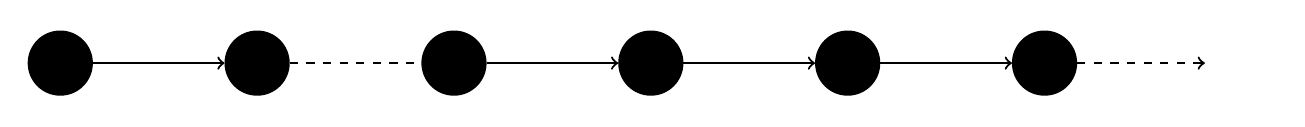
\begin{tikzpicture}[baseline=(current  bounding  box.center), thick]
\node [circle, draw, fill=black, minimum size=.8cm] (a1) at (0,0) {};
\node [circle, draw, fill=black, minimum size=.8cm] (a2) at (2.5,0) {};
\node [circle, draw, fill=black, minimum size=.8cm] (a3) at (5,0) {};
\node [circle, draw, fill=black, minimum size=.8cm] (a4) at (7.5,0) {};
\node [circle, draw, fill=black, minimum size=.8cm] (a5) at (10,0) {};
\node [circle, draw, fill=black, minimum size=.8cm] (a6) at (12.5,0) {};
\node [circle, minimum size=.9cm] (a7) at (15,0) {};

\draw[->] (a1) -- (a2); 
\draw[dashed] (a2) -- (a3);
\draw[->] (a3) -- (a4);
\draw[->] (a4) -- (a5);
\draw[->] (a5) -- (a6);
\draw[dashed, ->] (a6) -- (a7);
\end{tikzpicture}
\begin{table}[H]
%\centering
\hspace{1cm}\begin{tabular}{p{0.72cm}p{0.9cm}p{0.72cm}p{0.9cm}p{0.72cm}p{0.9cm}p{0.72cm}p{0.9cm}p{0.72cm}p{0.9cm}p{0.72cm}p{0.9cm}}
$\phi$ &  &$\phi$ & ... &  &  &  &  &  &  &  &  \\
$\psi$ &  &  &  &  &  &  &  &  &  &  &  \\
  &\textbf{or} & $\psi$ &  &  &  &  &  &  &  &  &  \\
  &  &  & \textbf{or} & $\psi$ &  &  &  &  &  &  & 
\end{tabular}
%\caption{}
\label{tab:Q2_1}
\end{table}
If $\phi$ is an invariant, then $\psi$ is true in some moment in time.\\

\item 
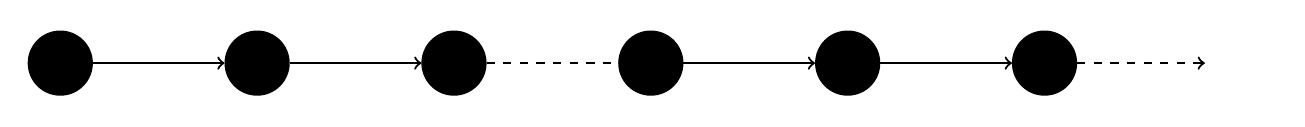
\begin{tikzpicture}[baseline=(current  bounding  box.center), thick]
\node [circle, draw, fill=black, minimum size=.8cm] (a1) at (0,0) {};
\node [circle, draw, fill=black, minimum size=.8cm] (a2) at (2.5,0) {};
\node [circle, draw, fill=black, minimum size=.8cm] (a3) at (5,0) {};
\node [circle, draw, fill=black, minimum size=.8cm] (a4) at (7.5,0) {};
\node [circle, draw, fill=black, minimum size=.8cm] (a5) at (10,0) {};
\node [circle, draw, fill=black, minimum size=.8cm] (a6) at (12.5,0) {};
\node [circle, minimum size=.9cm] (a7) at (15,0) {};

\draw[->] (a1) -- (a2); 
\draw[->] (a2) -- (a3);
\draw[dashed] (a3) -- (a4);
\draw[->] (a4) -- (a5);
\draw[->] (a5) -- (a6);
\draw[dashed, ->] (a6) -- (a7);
\end{tikzpicture}
\begin{table}[H]
%\centering
\hspace{1cm}\begin{tabular}{p{0.72cm}p{0.9cm}p{0.72cm}p{0.9cm}p{0.72cm}p{0.9cm}p{0.72cm}p{0.9cm}p{0.72cm}p{0.9cm}p{0.72cm}p{0.9cm}}
$\phi$ &  & $\phi$ &  & $\phi$ & ... &  &  &  &  &  &  \\
 &  & $\psi$ &  & $\psi$ & ... &  &  &  &  &  &  \\
 &  &  & \textbf{or} & $\psi$ &  & $\psi$ & ... &  &  &  &  \\
 &  &  &  &  & \textbf{or} & $\psi$ &  & $\psi$ & ... &  & 
\end{tabular}
%\caption{}
\label{tab:Q2_2}
\end{table}
If $\phi$ is an invariant, then from $i+1$ onwards, $\psi$ could become an invariant.\\

\item
\item
\item
\item
\item
\item
\end{enumerate}
\end{document}